\subsection{Decision Tree}

In our NLP problem, we also experimented with the DecisionTreeClassifier to improve our emotion classification model. The DecisionTreeClassifier is a model that creates a tree-like structure to make decisions based on the features of the input data.

During our experimentation, we focused on the parameter max\_depth to control the complexity of the tree. We found that the depth of the tree significantly impacted the model's performance.

Initially, without setting any maximum depth, the tree achieved an accuracy of 86\%. However, this unrestricted growth led to a highly complex model prone to overfitting.

Visualizing the decision trees helped us understand how the model splits the data at each node. Figure \ref{fig:complex_tree} shows a very detailed tree, while Figure \ref{fig:simple_tree} presents a more manageable structure.

We used accuracy to assess the model's performance and the overall accuracy with both max\_depth=3 and max\_depth=10 was around 16\% or less, highlighting the need for further optimization or potentially exploring other models. \autocite{decistion-tree}

\begin{figure}[H]
    \centering
    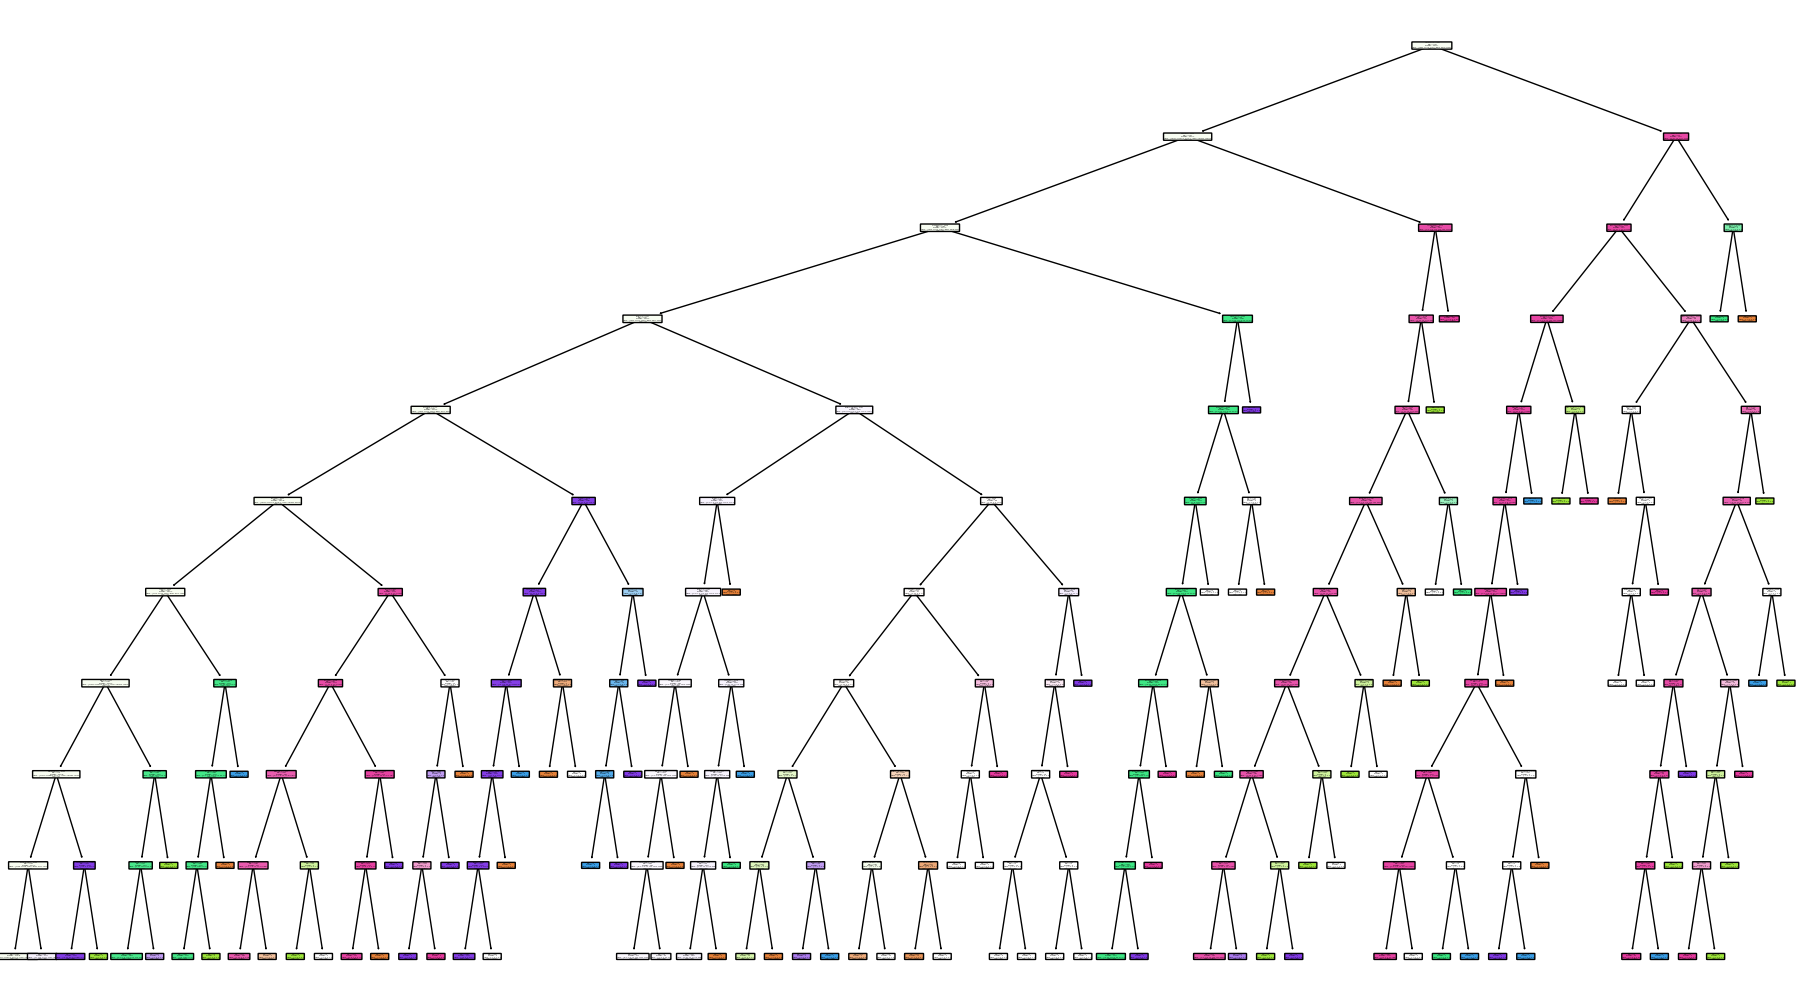
\includegraphics[width=0.8\columnwidth]{images/complex_tree.png}
    \caption{Decision tree illustrating overfitting with deep splits and numerous nodes. (max\_depth: 10)}
    \label{fig:complex_tree}
\end{figure}

\begin{figure}[H]
    \centering
    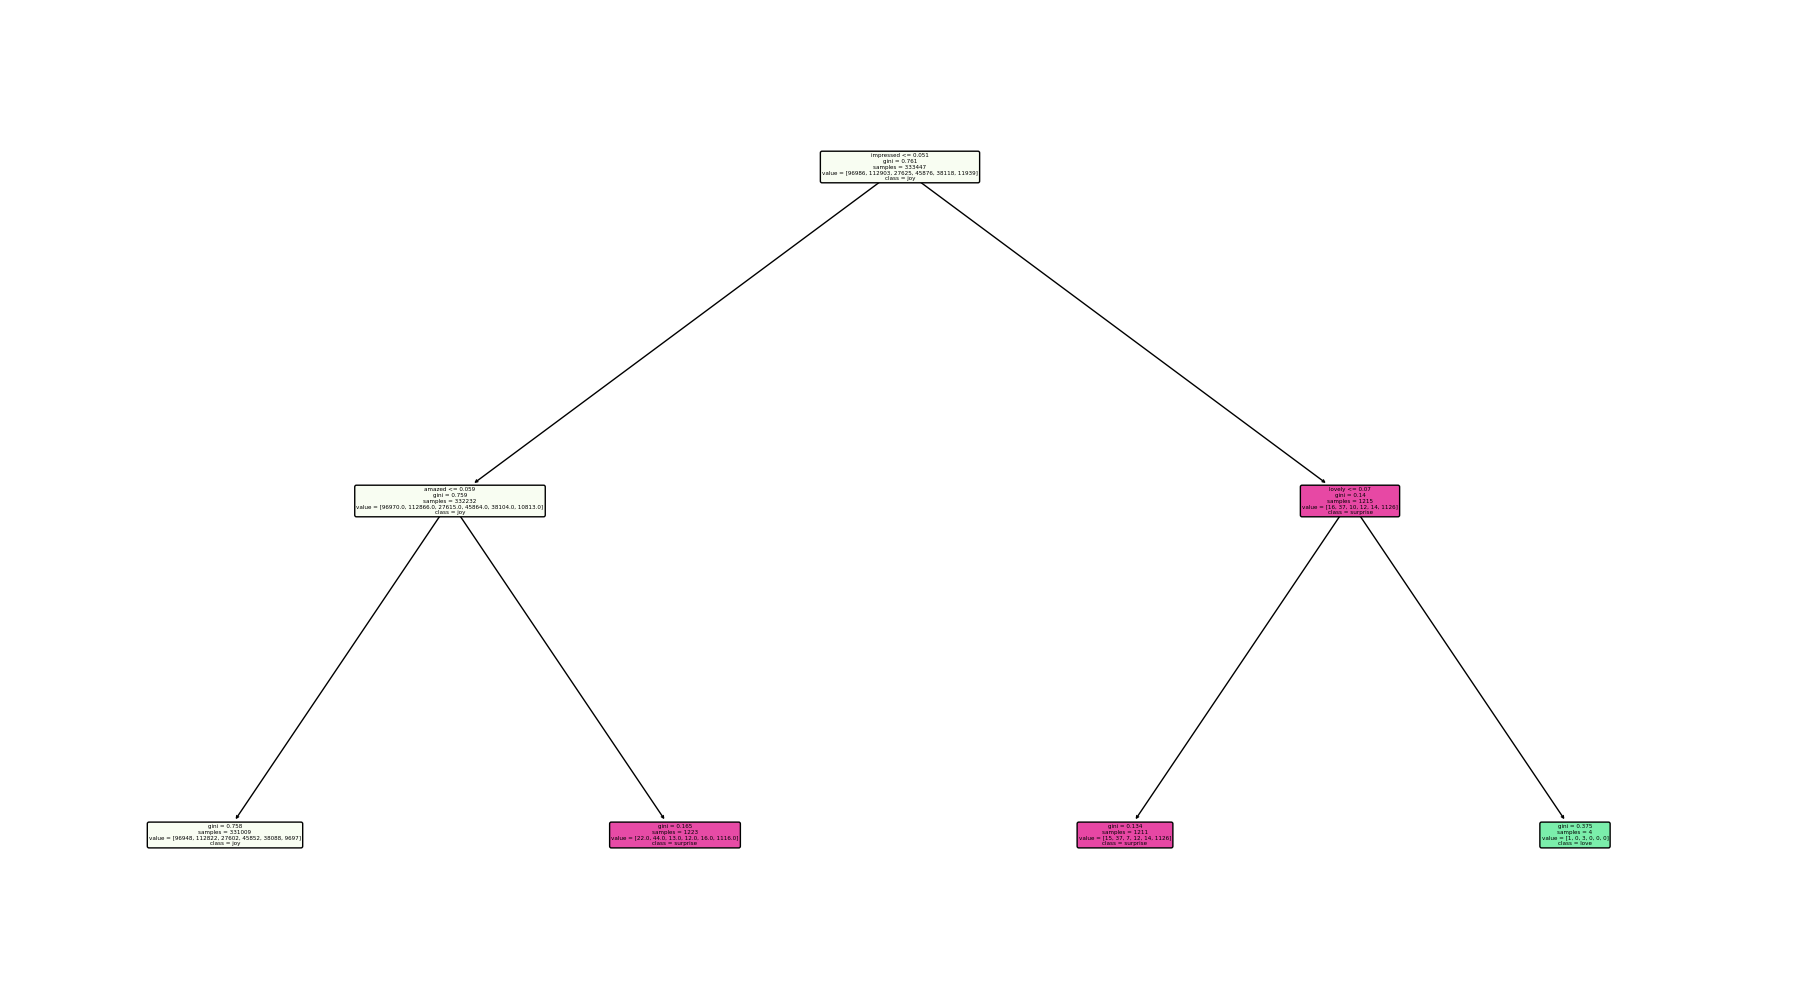
\includegraphics[width=0.8\columnwidth]{images/simple_tree.png}
    \caption{Pruned decision tree showing fewer levels and nodes. (max\_depth: 3)}
    \label{fig:simple_tree}
\end{figure}

% \begin{figure}[H]
%     \centering
%     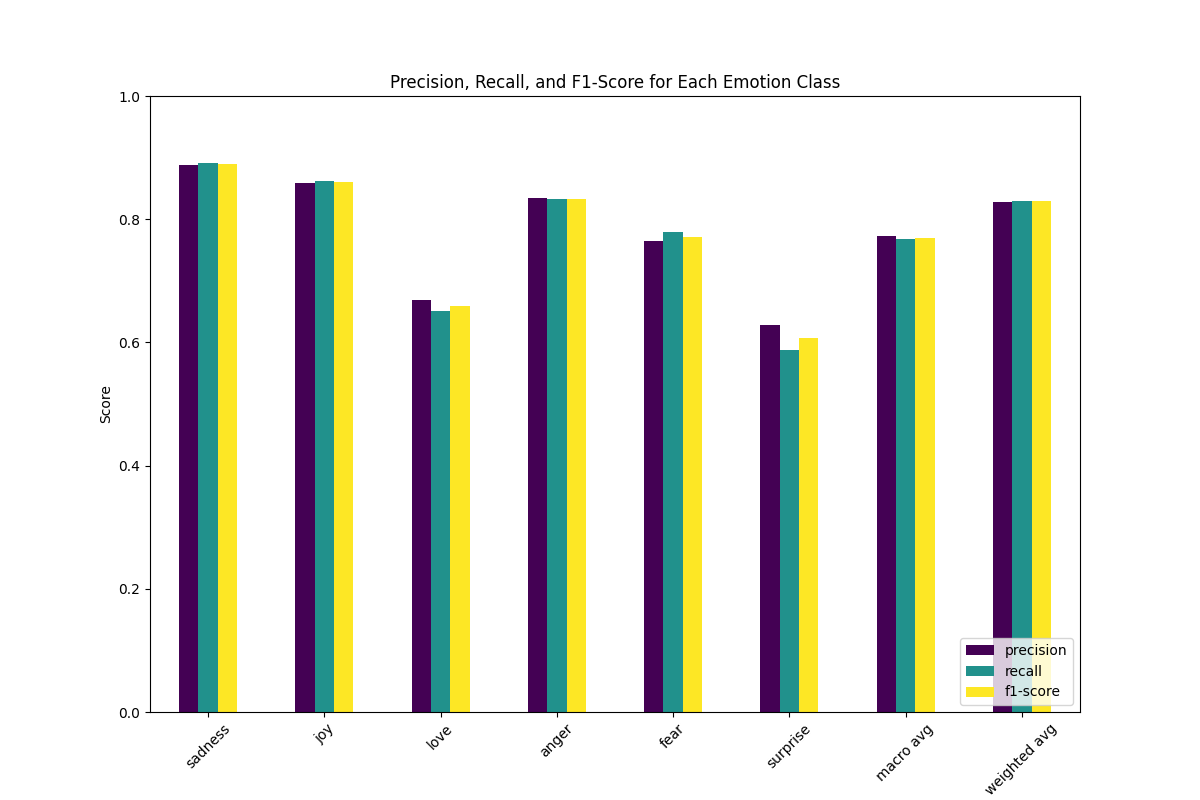
\includegraphics[width=1\columnwidth]{images/Classification_report_model2.png}
%     \caption{Classification report based on our decision tree classifier. Emotions showing a big variance in scores, indicating unreliable model predictions}
%     \label{fig:correlation_plot}    
% \end{figure}